% Chapter 1

\chapter{Introducción general} % Main chapter title

\label{Chapter1} % For referencing the chapter elsewhere, use \ref{Chapter1} 
\label{IntroGeneral}


%----------------------------------------------------------------------------------------

% Define some commands to keep the formatting separated from the content 
\newcommand{\keyword}[1]{\textbf{#1}}
\newcommand{\tabhead}[1]{\textbf{#1}}
\newcommand{\code}[1]{\texttt{#1}}
\newcommand{\file}[1]{\texttt{\bfseries#1}}
\newcommand{\option}[1]{\texttt{\itshape#1}}
\newcommand{\grados}{$^{\circ}$}

%----------------------------------------------------------------------------------------

%\section{Introducción}

%----------------------------------------------------------------------------------------
% \section{Resumen inicial{}}
En este capítulo se presentan las motivaciones que impulsaron el desarrollo del sistema, diseñado para automatizar la comunicación entre emprendedores y sus clientes. Se ofrece, además, una explicación detallada sobre qué son los chatbots y las razones por las que su uso resulta fundamental en este contexto. Finalmente, se describen los objetivos principales del trabajo, centrados en la facilidad de implementación y en la mejora de la eficiencia operativa, junto con el alcance definido durante la planificación.

\section{Motivación{}}

El sistema desarrollado en el presente trabajo surge de la necesidad de proporcionar a emprendedores una herramienta que les permita automatizar la comunicación con sus clientes de manera eficiente y personalizada. Esta herramienta les ofrece una ventaja competitiva al optimizar la gestión de sus interacciones con los usuarios y les permite mejorar la eficiencia operativa, además de reducir los costos asociados a la atención al cliente.


\subsection{¿Qué es un chatbot?}

Un chatbot es un programa de software que emplea técnicas de Procesamiento del Lenguaje Natural (PLN) \citep{ibm-pln}, para interpretar y contestar automáticamente las consultas de los usuarios de manera coherente y eficiente. Esto facilita la automatización de interacciones comunes y mejora la experiencia del cliente.


\subsection{¿Por qué un chatbot?}

A continuación, se destacan algunas de las razones principales por las que un chatbot es la solución ideal para este trabajo:

\begin{itemize}
    \item Disponibilidad 24/7: los chatbots están disponibles en todo momento, lo que les permite a las empresas atender consultas de sus clientes a cualquier hora del día.
    
    \item Reducción de costos: al automatizar la atención al cliente, los chatbots ayudan a las empresas a reducir los costos asociados al personal humano sin comprometer la calidad del servicio.
    
    \item Recolección de datos valiosos: los chatbots pueden recopilar y analizar información relevante sobre las interacciones con los clientes, lo que les permite a las empresas ajustar sus estrategias de manera eficiente.
    
    \item Optimización de tiempos de respuesta: la capacidad de generar respuestas inmediatas en función de consultas predefinidas optimiza los tiempos de respuesta.
\end{itemize}

% \subsection{Guía matemática rápida para \LaTeX{}}

% Si estás escribiendo un documento con mucho contenido matemático, entonces es posible que desees leer el documento de la AMS (American Mathematical Society) llamado, \enquote{A Short Math Guide for \LaTeX{}}. Se puede encontrar en línea en el siguiente link: \url{http://www.ams.org/tex/amslatex.html} en la sección \enquote{Additional Documentation} hacia la parte inferior de la página.


%----------------------------------------------------------------------------------------

\section{Alcance y objetivos{}}

\subsection{Objetivos principales}

El trabajo se enfoca en tres objetivos principales que se interrelacionan para ofrecer una solución integral a pequeños emprendedores. Cada uno de estos objetivos está orientado a asegurar que la herramienta sea accesible, fácilmente implementable y de bajo costo, para garantizar una experiencia eficiente y optimizada para las empresas que la adopten. 
 
A continuación, se detallan los objetivos principales:


\begin{itemize}
    \item Proporcinar acceso a pequeños emprendedores: desarrollar un sistema que sea de fácil adopción y pueda ser utilizado por pequeñas empresas, independientemente de sus conocimientos técnicos.
    
    \item Garantizar una fácil implementación: diseñar una solución replicable, de modo que cualquier empresa pueda contar con el chatbot simplemente al proporcionar el contexto necesario para su entrenamiento. No será necesario disponer de infraestructura compleja ni personal especializado.
    
    \item Reducir el costo de mantenimiento: proporcionar una herramienta con un bajo costo de mantenimiento, tanto en términos económicos como de tiempo, para que los emprendedores puedan centrarse en su negocio principal.
    
\end{itemize}


% Incluir aquí el gráfico de Venn que detalle la relación de los objetivos principales.
% \includegraphics[width=\textwidth]{ruta/al/grafico_venn.png}

\begin{figure}[htbp]
  \centering
  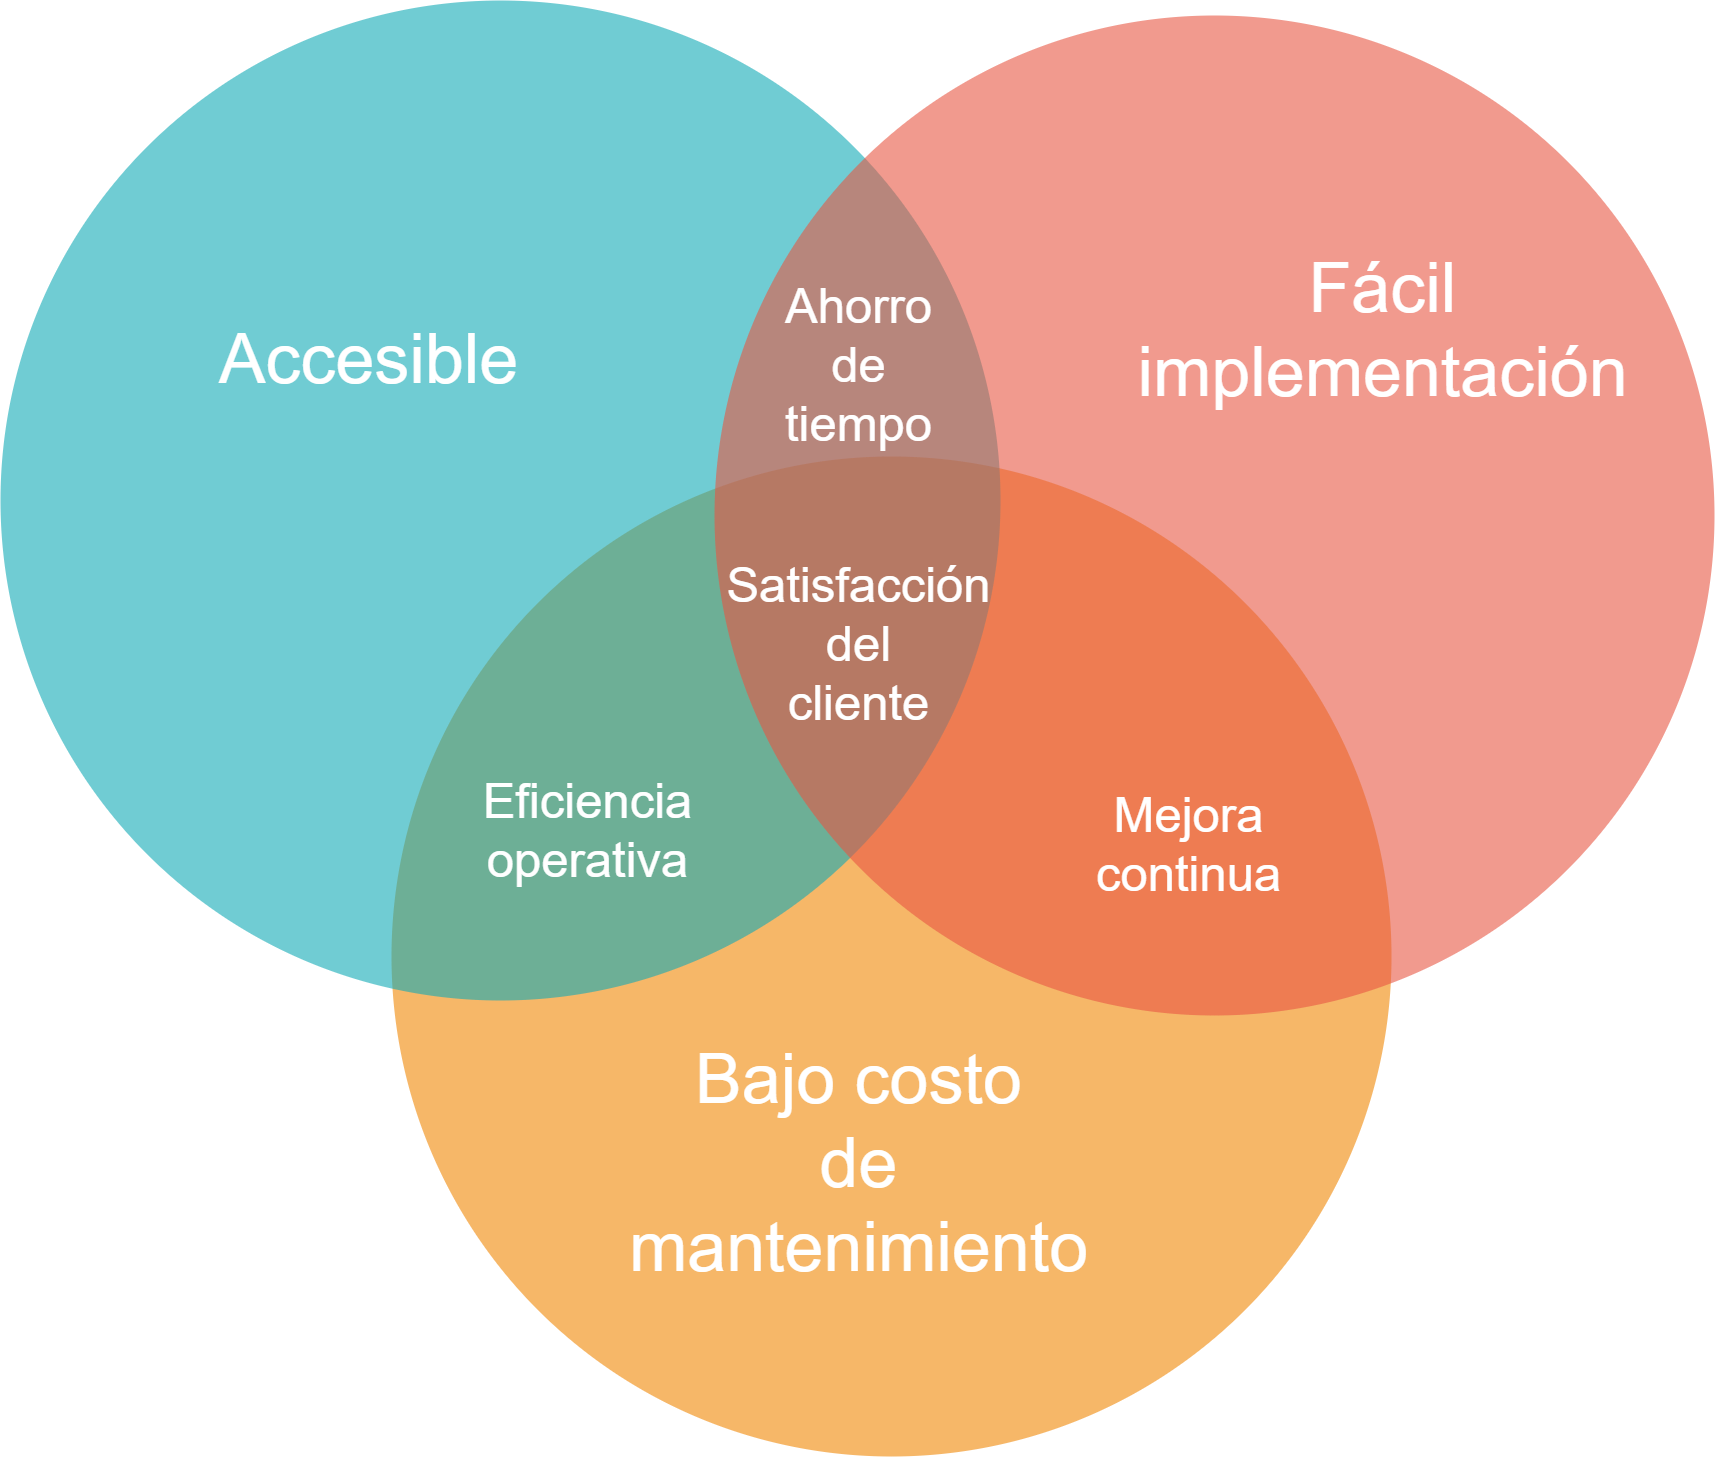
\includegraphics[width=.75\textwidth]{./Figures/Venn_objetivos.png}
  \caption{Relación entre los objetivos centrales.}
  \label{fig:objetivos_venn}
\end{figure}

\newpage % agrego un salto de página 
\subsection{Alcance del trabajo}

Durante la planificación del trabajo se propusieron las siguientes actividades:

\begin{itemize}
    \item Diseño, desarrollo e implementación de un \textit{pipeline} completo para la creación y gestión de chatbots basados en PLN, con capacidad de aprendizaje continuo.
    \item Desarrollo de algoritmos para el preprocesamiento de información y generación de respuestas relevantes y coherentes.
    \item Establecimiento de métricas y procedimientos de evaluación para medir la calidad y eficacia de las respuestas del chatbot.
    \item Implementación de un sistema de retroalimentación que utilice los datos de interacciones con usuarios para mejorar el rendimiento del modelo.
\end{itemize}

\vspace{0.5cm} % Esto añade un pequeño espacio vertical (medio centímetro)

El presente trabajo excluye: 
\begin{itemize}
    \item Desarrollo de interfaces de usuario avanzadas, por fuera de las básicas necesarias para probar el pipeline.
    \item Integración con sistemas externos, como bases de datos o plataformas de gestión de clientes.
    \item Implementación del sistema en un entorno productivo.
    \item Actividades de marketing o promoción del producto final.
\end{itemize}


 

%----------------------------------------------------------------------------------------
% \newpage % agrego un salto de página 

 

\section{Estado del arte}

Los chatbots se han integrado en numerosos aspectos de la vida diaria y en diversos canales de comunicación. Se encuentran presentes en redes sociales como Facebook e Instagram, donde facilitan la interacción con empresas. Además, muchas organizaciones y entidades gubernamentales, han implementado chatbots para mejorar la atención al ciudadano. Plataformas como IBM Watson, Google Dialogflow y Microsoft Bot Framework permiten a las empresas crear chatbots personalizados con gran flexibilidad.

\subsection{Recursos para chatbots}

\subsubsection{Servicios basados en APIs}
Los servicios basados en API\footnote{API (Interfaz de Programación de Aplicaciones) es un conjunto de reglas y protocolos que permite que diferentes aplicaciones se comuniquen entre sí.} simplifican la implementación de chatbots al ofrecer interfaces estandarizadas para acceder a funcionalidades avanzadas. Estos servicios permiten una mayor personalización y flexibilidad en el diseño de chatbots, que facilitan la integración con otros sistemas y plataformas. La utilización de APIs permite a las empresas adaptar las soluciones a sus necesidades específicas sin necesidad de desarrollar toda la infraestructura desde cero.


\subsubsection{Modelos locales}
Los modelos locales como Llama 3.1, Phi 3, Gemma y Mistral son soluciones robustas que operan sin depender de servicios externos. Cada uno de estos ofrece características y ventajas específicas, como mayor control sobre los datos y la posibilidad de operar en entornos con restricciones de privacidad. Su uso es particularmente valioso cuando se requiere un alto nivel de personalización y seguridad en la gestión de datos.


\subsection{Tendencias actuales}
Cada vez más empresas optan por utilizar servicios basados en API, que han hecho más accesible y económico el despliegue de chatbots sofisticados. Estas herramientas simplifican la implementación y permiten la creación rápida de soluciones adaptadas a las necesidades específicas de cada empresa o entidad. Aunque los modelos locales son valiosos por su robustez y capacidad para operar sin depender de servicios externos, son útiles especialmente cuando se requiere un mayor control o confidencialidad.


 